\section{Plant layout}

\subsection{Plant location \& general plot layout}

Nitroma’s plant site will be located in Nanjing Jiangbei New Material Science Park in Nanjing, Jiangsu. One of the main advantages of this location is the shared utilities (including power, steam, water and recycling facilities), which are available to facilities in the area. \cite{independent_commodity_intelligence_services_china_2007}. The site lies on the northern banks of the Yangtze River, situated approximately 30km from the city centre, a significant distance between the site and the residential areas \cite{zeng_divergent_2011}. The location allows close access to the harbour for imports and exports, with the river providing a source of cooling water supply, without the need for a cooling water tower.

\begin{wrapfigure}{R}{0.6\linewidth}
\centering
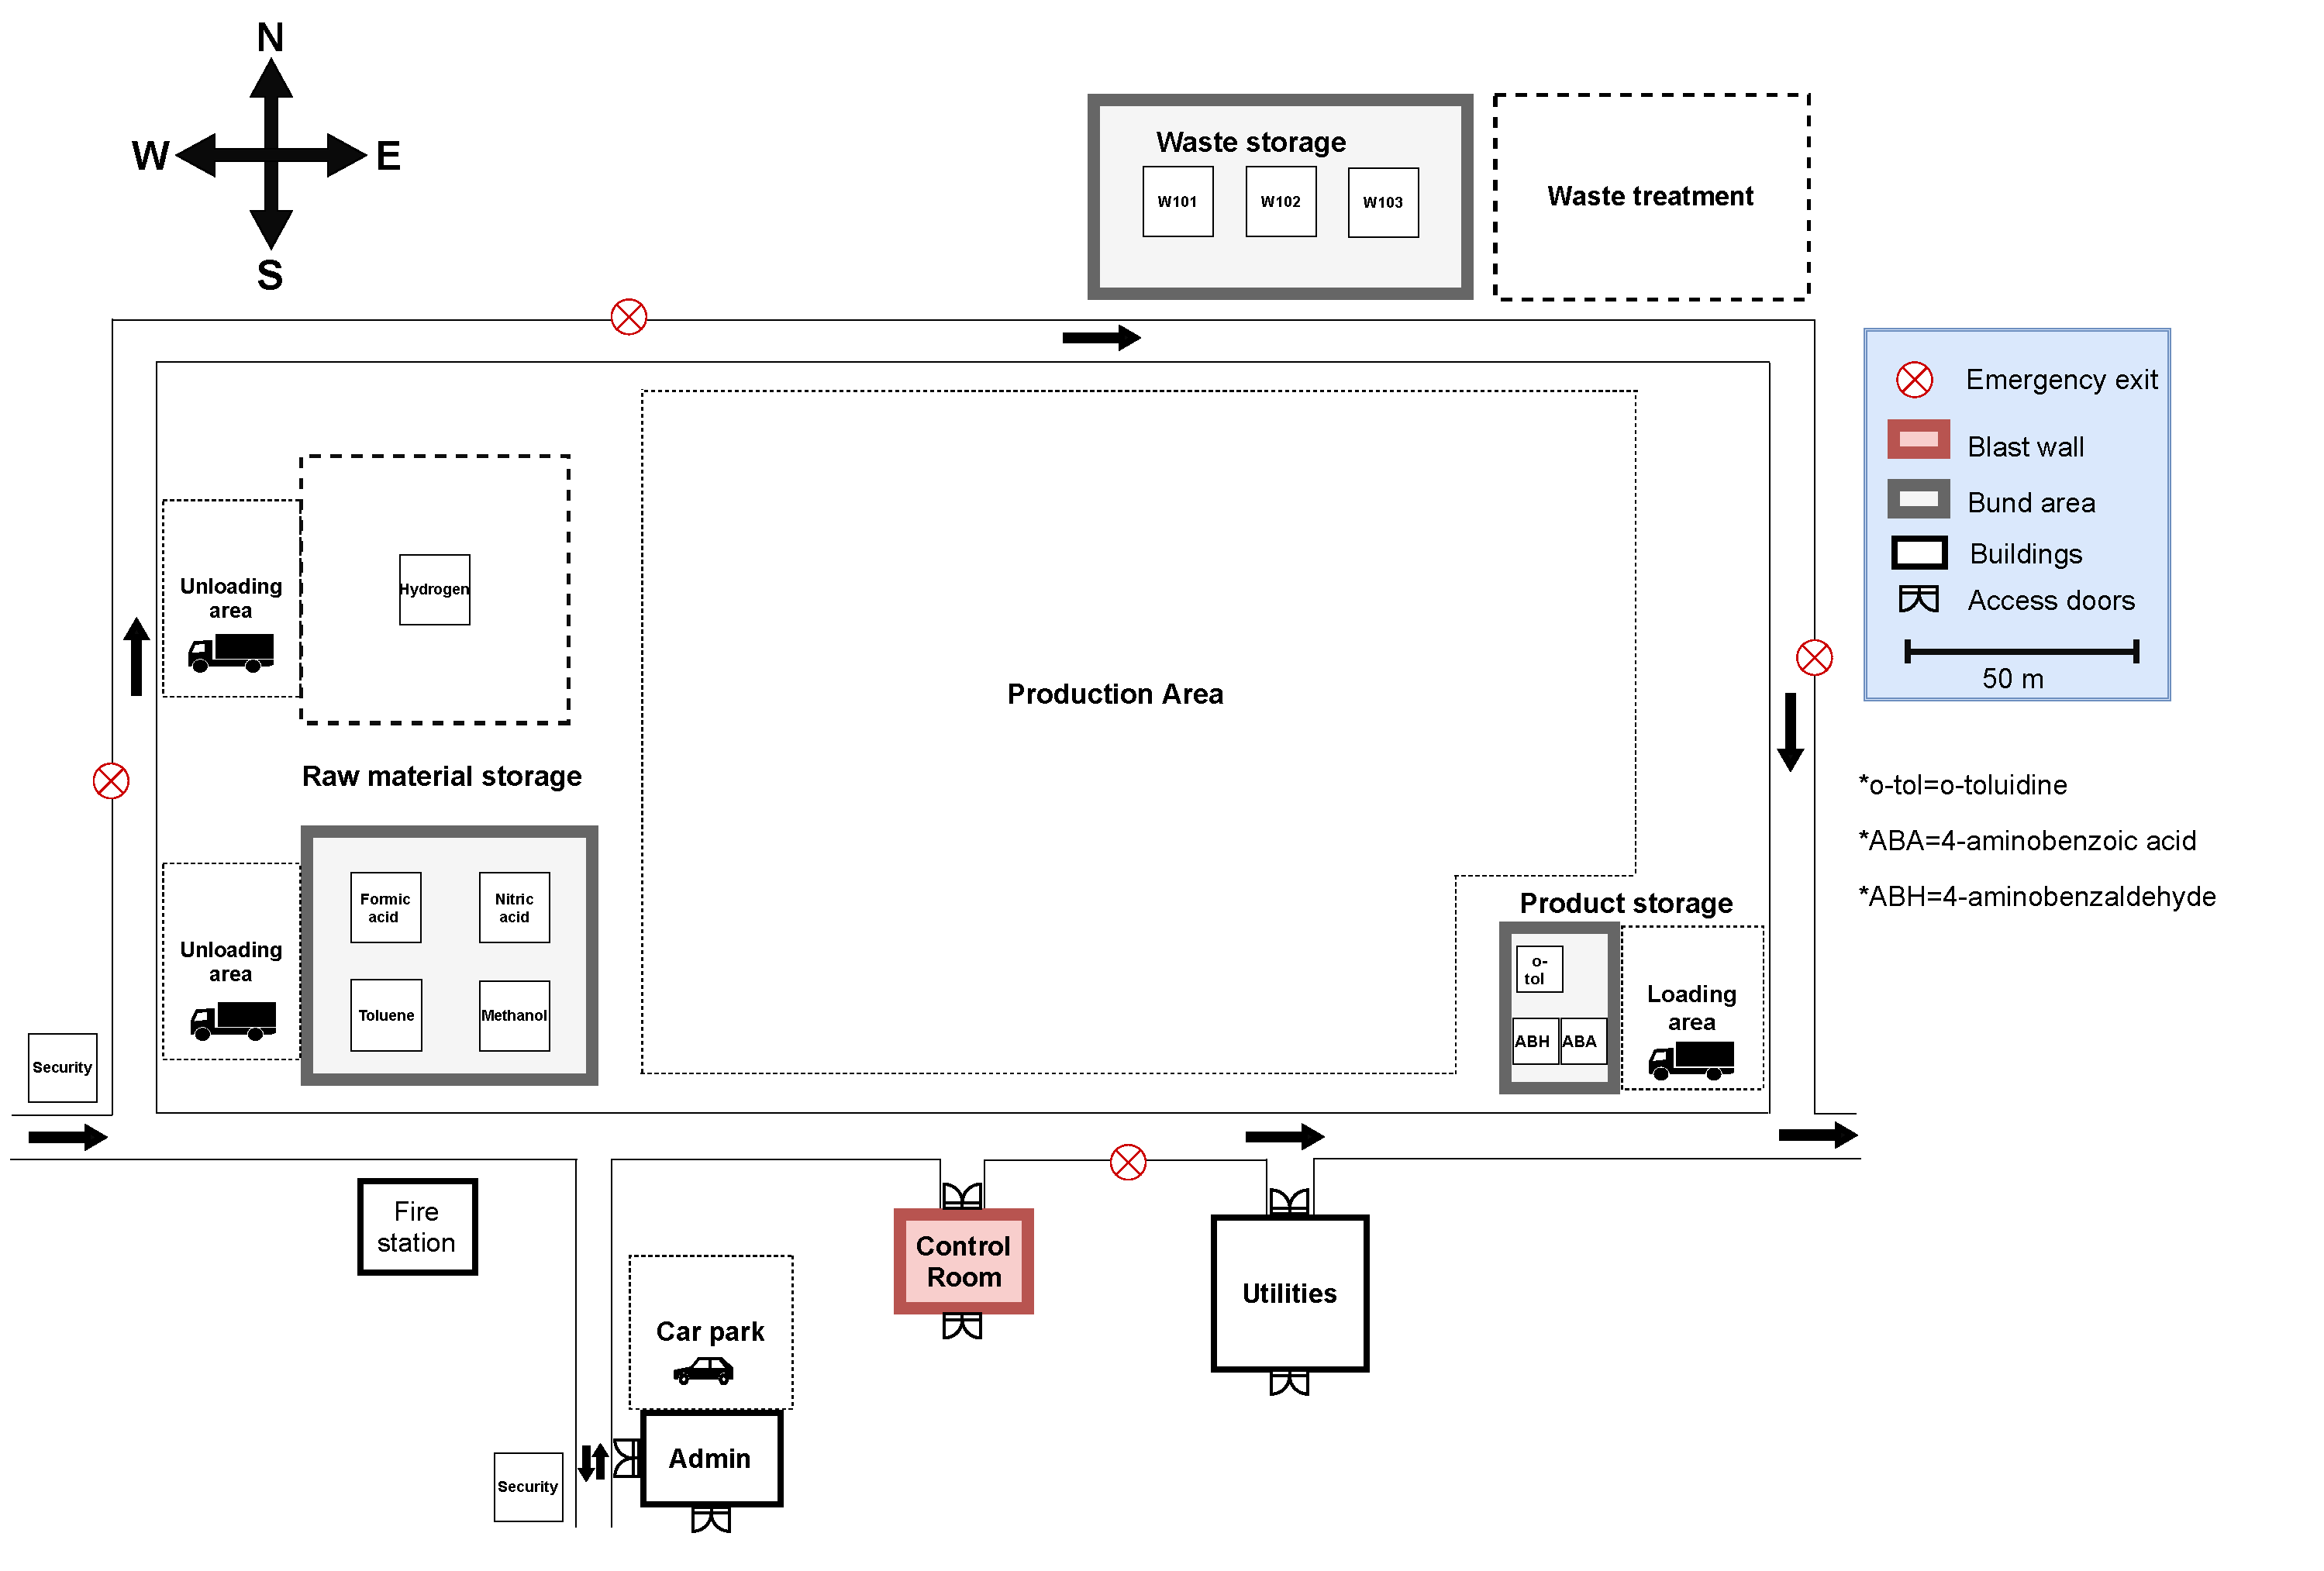
\includegraphics[width=\linewidth]{chapters/5-safety-layout-environment/figures/Plant layout 3.pdf}
\caption{Site Layout}
\label{fig:site}
\end{wrapfigure}

The initial design of the plant layout began with the block layout methodology, providing a simple visualisation of various areas which are segregated according to associated risks and spacing requirements \cite{center_for_chemical_process_safety_site_2010}. The site will be spilt into three sectors. The first sector will hold the main production site. As this is the sector associated with the highest risk, it has been isolated from other areas of the plant. The second sector will consist of the control room, the storage units and the waste treatment site. The last sector will facilitate the administrative building, car park and an onsite fire station. Alongside the main entrance routes, there will also be evacuation sites in each sector for emergencies. There are at least two access doors for all buildings on site \cite{aiche_dows_1994}. 

\subsection{Production site}

A detailed view of the production area is shown in \cref{fig:detailed_layout}. The production site of the plant will consist of 5 major sections:

\begin{itemize}
    \item Toluene nitration
    \item 2-Nitrotoluene reduction 
    \item 4-Nitrotoluene oxidation 
    \item 4-Nitrobenzoic acid reduction 
    \item 4-Nitrobenzaldehyde reduction 
\end{itemize}

As mentioned previously, the production site will be isolated from other areas of the plant, as this section holds the highest risk of fires, explosions and release of toxic materials occurring. The equipment layout for the production area in Section \Cref{fig:detailed_layout} was designed based on the principle of flow. Major process units were arranged in the same order as they are seen on the process flow diagram \cite{mannan_lees_2012}. This minimises transport of materials and increases material handling efficiency, which is favourable from an economical and safety perspective.  

\subsection{Waste treatment site}

\begin{wrapfigure}{R}{0.3\linewidth}
\centering
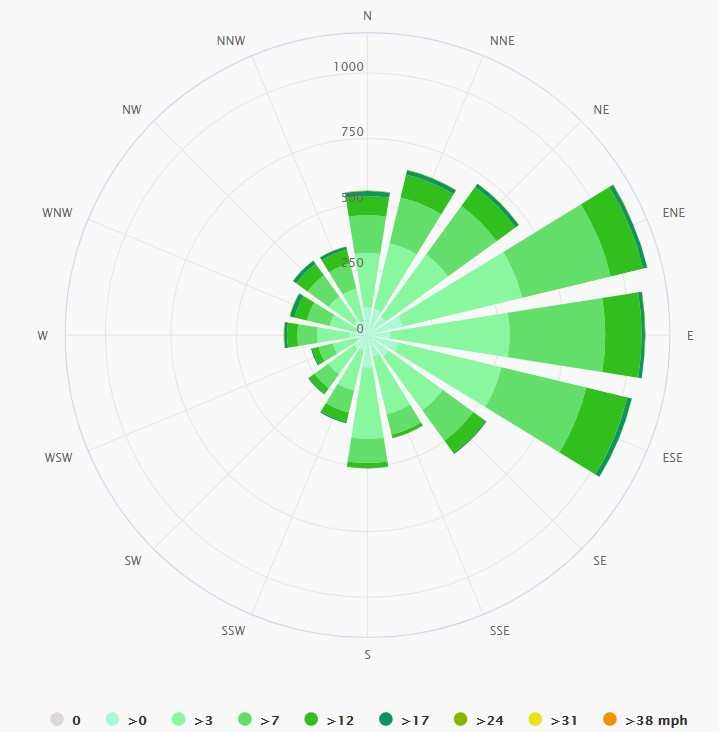
\includegraphics[width=\linewidth]{chapters/5-safety-layout-environment/figures/Windrose_profile.jpg}
\caption{Wind profile in Nanjing, China \cite{meteoblue_climate_nodate}}
\label{fig:wind}
\end{wrapfigure}


\Cref{fig:wind} shows the wind profile in Nanjing, China with wind predominantly acting from west to east. Since the wastewater treatment units include stacks with gaseous emissions, it was sited beside the production area, further away from the control and admin buildings. It was also placed downwind to the wind profile so that the plumes will be moving away from the plant site. 

\subsection{Control room}

The control room is located outside the main production site, as recommended by the health and safety executive (HSE) \cite{health_and_safety_executive_control_nodate}. The control room will be separated from the plant by a distance of 30 m according to the recommended minimum distance \cite{mannan_lees_2012}. To ensure safety of operators in the control room, the windows will be sealed to prevent the influx of harmful gases that may be released. The control room will have blast proof walls with windows constructed of polycarbonate glass, to protect the workers in the event of overpressure \cite{health_and_safety_executive_control_nodate}. The control room will also have adequate lighting, situated away from regions of a high noise level that may distract operators.

\subsection{Storage Units}

There will be three storage categories: raw material, product and waste. There are general storage rules that will apply to all three of these storage sections: 

\begin{itemize}
    \item Adequate spacing between flammable materials and oxidising materials.
    \item Flammable materials will be stored well below their respective auto-ignition temperature and below their flash points.
\end{itemize}

Storage will be segregated from the production area to avoid the risk of fire propagating from the production area to the storage tanks \cite{mannan_lees_2012}. The raw material storage tanks were placed closer to the equipment utilising it and the product storage tanks were placed closer to the end of the production area for easy access. The waste storage was placed in closer proximity to the waste treatment plant. The raw material loading and product unloading terminals was separated. Due to the hazardous nature of the substances they were placed away from the entrance to the plant. All storage areas are placed at least 15 m away from the production area. 

Raw materials (excluding hydrogen), products and waste will be stored in atmospheric storage tanks provided with full bund to prevent spillage of toxic materials. Hydrogen would be stored in a pressure container since it will be at 5 atm, which is above atmospheric pressure.


\subsection{Utility room}
This room contains essential ancillary services needed for the plant process. This includes back-up power generation, water storage for general use, cooling water, steam and refrigeration. 

\subsection{Administrative building}

As the low-hazard section of the plant, the administrative building has been placed furthest away from the production site, waste treatment and storage sites, minimising consequential effects workers may endure in the event of a fire, explosion or toxic release that occurs on the more operational sectors. The administration building is placed in the upwind direction. Within the administrative building, there will be offices and conference rooms, a cafeteria, lavatories, and a medical centre. \cite{sinnott_coulson_2005}. 

\subsection{Dow's Fire and Explosion Index (F\&EI)}
The F\&EI were calculated for only major process units such as reactors, separators, waste process units and storage tanks containing flammable or unstable materials. Results are summarised in \cref{tab:radius} The highest Material Factor (MF) for a component in the mixture was used for each process unit. Then, General Process Hazards Factor ($F_1$) and Special Process Hazards Factor ($F_2$) were determined. The product of the two factors determined the Process Unit Hazards Factor ($F_3$). F\&EI was determined from the product of $F_3$ and MF. According to the Dow's F\&EI, the Radius of Exposure, in metres, was determined by multiplying the F\&EI by a factor of 0.256 \cite{aiche_dows_1994}.This was used in the plant layout to determine the separation distance between major process units.    